% !TEX root = sirocco-main.tex

\section{Introduction}

A dominating set in an undirected and simple graph $G$ is a set
$D\subseteq V(G)$ such that every vertex $v\in V(G)$ either belongs
to $D$ or has a neighbor in $D$. The \textsc{Minimum Dominating Set} problem takes as input a graph $G$ and the objective
is to find a minimum size dominating set of~$G$. The decision
problem whether a graph admits a dominating set of size $k$
is NP-hard~\cite{karp1972reducibility} and this even holds in
very restricted settings, e.g. on planar graphs of maximum degree
$3$~\cite{garey1979computers}.

Consequently, attention
shifted from computing exact solutions to approxi\-mating
near optimal dominating sets. The simple greedy algorithm computes
an $\ln n$ approximation (where $n$ is number of vertices
of the input graph)
of a minimum dominating set \cite{johnson1974approximation,lovasz1975ratio}, and for
general graphs this algorithm is near optimal -- it is NP-hard
to approximate minimum dominating sets within factor
$(1-\epsilon)\ln n$ for every $\epsilon>0$~\cite{dinur2014analytical}.

Therefore, researchers tried to identify restricted
graph classes where better (sequential) approximations are possible. The problem
admits a PTAS on classes with sub\-exponential expansion~\cite{har2017approximation}. Here, expansion refers to the edge
density of bounded depth minors, which we will define in
detail below. Important examples of classes with subexponential
expansion include the class of planar graphs and more generally
classes that exclude some fixed graph as a minor. The dominating
set problem admits a constant factor approximation on classes of
bounded degeneracy (equivalently, of bounded arboricity)~\cite{bansal2017tight,lenzen2010minimum}
and an $\Oof(\ln \gamma)$ approxi\-mation (where~$\gamma$ denotes the size
of a minimum dominating set) on classes of bounded VC-dimension~\cite{bronnimann1995almost,even2005hitting}. In fact, the greedy
algorithm can be modified to yield a constant factor approximation on
graphs with bounded degeneracy~\cite{jones2017parameterized} and an $\Oof(\ln \gamma)$
approximation on biclique-free graphs (graphs that exclude some fixed
complete bipartite graph $K_{t,t}$ as a subgraph)~\cite{siebertz2019greedy}. However, it is unlikely
that polynomial-time constant factor approximations exist even on
$K_{3,3}$-free graphs~\cite{siebertz2019greedy}.
The general goal in this line of research is to identify the broadest
graph classes on which the dominating set problem (or other important
problems that are hard on general graphs) can be approximated
efficiently with a certain guarantee on the approximation factor.
These limits of tractability are often captured by abstract notions, such
as expansion, degeneracy or VC-dimension of graph classes.


\medskip
In this paper we study the distributed time complexity of finding
dominating sets in the classic LOCAL model of distributed computing,
which can be traced back at least to the seminal work of Gallager,
Humblet and Spira~\cite{gallager1983distributed}. In this model, a
distributed system is modeled by an undirected (connected) graph~$G$,
in which every vertex represents a computational entity of the network and every edge represents a bidirectional communication channel. The vertices are equipped with unique identifiers.
In a distributed algorithm, initially, the nodes have no knowledge about
the network graph. They must then communicate and coordinate
their actions by passing messages to one another in order to achieve
a common goal, in our case, to compute a dominating set of the
network graph. The LOCAL model focuses on the aspects of
communication complexity and therefore the main measure for
the efficiency of a distributed algorithm is the number of communication
rounds it needs until it returns its answer.

Kuhn et al.~\cite{KuhnMW16} proved that in~$r$ rounds on an~$n$-vertex graphs of maximum degree
$\Delta$ one can approximate minimum dominating sets only within a factor $\Omega(n^{c/r^2}/r)$
and~$\Omega(\Delta^{1/(r+1)}/r)$, respectively, where~$c$ is a constant.
This implies that, in general, to achieve a constant approximation ratio,
we need at least $\Omega(\sqrt{\log
    n/\log \log n})$ and~$\Omega(\log \Delta/\log \log \Delta)$ communication rounds, respectively.
Kuhn et al.~\cite{KuhnMW16} also presented a~$(1+\epsilon)\ln \Delta$-approximation in that runs in $\Oof(\log(n)/\epsilon)$ rounds for any~$\epsilon>0$,
Barenboim et al.~\cite{barenboim2018fast}
presented a deterministic $\Oof((\log n)^{k-1})$-time algorithm that provides an
$\Oof(n^{1/k})$-approximation, for any integer parameter~$k \ge 2$.
More recently, the combined works of Rozhon, Ghaffari, Kuhn, and Maus~\cite{DBLP:conf/stoc/GhaffariKM17,DBLP:conf/stoc/RozhonG20}
provide an algorithm computing a $(1+\epsilon)$-approximation of the dominating set
in poly$(\log(n)/\epsilon)$ rounds~\cite[Corollary 3.11]{DBLP:conf/stoc/RozhonG20}. 

For graphs of degeneracy~$a$ (equivalent to arboricity up to factor $2$),
Lenzen and Wattenhofer~\cite{lenzen2010minimum}
provided an algorithm that achieves a factor~$\Oof(a^2)$ approximation
in randomized time~$\Oof(\log n)$, and a deterministic~$\Oof(a \log
\Delta)$ approximation algorithm
with $\Oof(\log \Delta)$ rounds. Graphs of bounded degeneracy include all graphs that exclude a fixed graph as a (topological) minor and in particular, all planar graphs and any class of bounded genus.

Amiri et al.~\cite{akhoondian2018distributed} provided a deterministic
$\Oof(\log n)$ time constant factor approximation algorithm on
classes of bounded expansion (which extends also to connected
dominating sets).
Czygrinow et al.~\cite{czygrinow2008fast} showed
that for any given~\mbox{$\epsilon>0$}, $(1+\epsilon)$-approximations of a maximum independent
set, a maximum matching, and a minimum dominating set, can be computed in
$\Oof(\log^* n)$ rounds in planar graphs, which is asymptotically optimal~\cite{lenzen2008leveraging}.

Lenzen et al.~\cite{lenzen2013distributed} proposed a constant factor
approximation on planar graphs that can be computed in a
constant number of communication rounds (see also~\cite{wawrzyniak2014strengthened}
for a finer analysis of the approximation factor).
Wawrzyniak~\cite{wawrzyniak2013brief} showed
that message sizes of $\mathcal{O}(\log n)$ suffice to give a
constant factor approximation on planar graphs in a constant number
of rounds.
In terms of lower bounds, Hilke et al.~\cite{hilke2014brief} showed that there is no
deterministic local algorithm (constant-time distributed graph algorithm) that
finds a~$(7-\epsilon)$-approximation of a minimum dominating set on
planar graphs, for any positive constant~$\epsilon$.

The results for planar
graphs were gradually extended to classes with bounded genus~\cite{akhoondian2016local,amiri2016brief}, classes with sublogarithmic expansion~\cite{amiri2019distributed} and eventually by Czygrinow et al.~\cite{czygrinow2018distributed} to classes with excluded topological minors.
Again, one of the main goals in this line of research is to find the most general
graph classes on which the dominating set problem admits a constant
factor approximation in a constant number of rounds.


\begin{figure}[h!]
\begin{center}
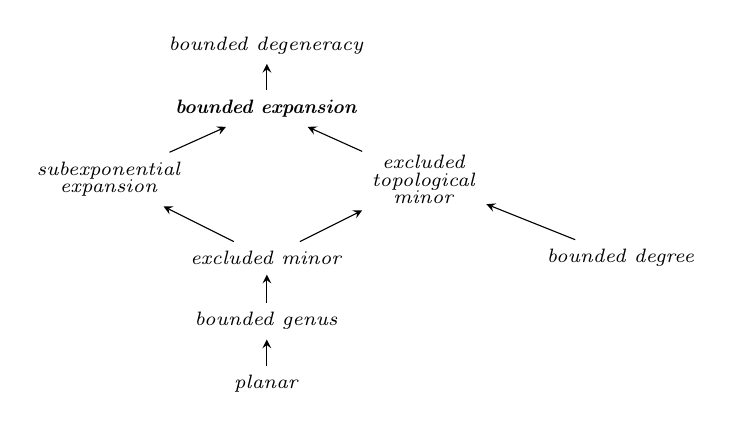
\begin{tikzpicture}

\node (bd-deg) at (11,-2.7) {\scriptsize\textit{bounded degree}};
\node[align=center] (topminor) at (8.5,-1.7) {\scriptsize\textit{excluded}\\[-2mm]\scriptsize\textit{topological}\\[-2mm] \scriptsize\textit{minor}};
\node[align=center] (sublog) at (4.5,-1.7) {\scriptsize\textit{subexponential}\\[-2mm]\scriptsize\textit{expansion}};
\node (bd-exp) at (6.5,-0.8) {\scriptsize\textbf{\textit{bounded expansion}}};
\node (degenerate) at (6.5,0) {\scriptsize\textit{bounded degeneracy}};
\node (planar) at (6.5,-4.3) {\scriptsize\textit{planar}};
\node (genus) at (6.5,-3.5) {\scriptsize\textit{bounded genus}};
\node (minor) at (6.5,-2.7) {\scriptsize\textit{excluded minor}};

%%%%%%%%%%%%%%%% Arrows %%%%%%%%%%%%%%%%

\draw[->,>=stealth] (planar) to (genus);
\draw[->,>=stealth] (genus) to (minor);
\draw[->,>=stealth] (minor) to (topminor);
\draw[->,>=stealth] (topminor) to (bd-exp);
\draw[->,>=stealth] (bd-deg) to (topminor);
\draw[->,>=stealth] (minor) to (sublog);
\draw[->,>=stealth] (sublog) to (bd-exp);
%\draw[->,>=stealth] (topminor) to[bend right=10] (bd-exp.east);
\draw[->,>=stealth] (bd-exp) to (degenerate);

\end{tikzpicture}
\end{center}
\caption{Inclusion diagram of the mentioned graph classes. }
\end{figure}\label{fig:classes}

\vspace{-3mm}
We take a step towards this goal and generalize the result of
Czygrinow et al.~\cite{czygrinow2018distributed} to classes of bounded
expansion. The notion of bounded expansion was introduced
by Ne\v{s}et\v{r}il and Ossona de Mendez~\cite{nevsetvril2008grad} and
offers an abstract definition of uniform sparseness in graphs. It is based on bounding the density of shallow minors. Intuitively, while
a minor is obtained by contracting arbitrary connected subgraphs of a graph
to new vertices, in an $r$-shallow minor we are only allowed to contract
connected subgraphs of radius at most~$r$.

A class of graphs has
bounded expansion if for every radius $r$ the set of all \mbox{$r$-shallow}
minors has edge density bounded by a constant depending only on~$r$.
We write $\nabla_r(G)$ for the maximal edge density of an
$r$-shallow minor of a graph~$G$.
Of course, every class~$\Cc$ that excludes a fixed graph $H$ as
a minor has bounded expansion. For such classes there exists an
absolute constant
$c$ such that for all $G\in\Cc$ and all~$r$
we have $\nabla_r(G)\leq c$.
Special cases are the class of
planar graphs, every class of graphs that can be drawn
with a bounded number of crossings, and every class of graphs
that embeds into a fixed surface.
Every class of intersection graphs of low density objects in low
dimensional Euclidean space has polynomial expansion, that is, the function~$\nabla_r$ is bounded polynomially in $r$ on $\Cc$. Also
every class $\Cc$ that excludes a fixed graph $H$ as
a topological minor has bounded expansion.
Important special cases are classes of
bounded degree and classes of graphs that can be drawn
with a linear number of crossings
Further examples include
classes with bounded queue-number, bounded stack-number or bounded
non-repetitive chromatic number
and the class of Erd\"os-R\'enyi random graphs with
constant average degree $d/n$, $G(n,d/n)$, has
asymptotically almost surely bounded expansion. See \cite{har2017approximation,nevsetvril2012characterisations} for all
these examples.

Hence, classes of bounded expansion are much more general than
classes excluding a topological minor. On the other hand, maybe
not surprisingly, when performing local
computations, it is not properties of minors or topological minors, but
rather of shallow minors that allow the necessary combinatorial arguments
in the algorithms. This observation was already made in the study of the kernelization complexity of dominating set on classes of sparse graphs \cite{DrangeDFKLPPRVS16,eiben2019lossy,EickmeyerGKKPRS17,FabianskiPST19,kreutzer2018polynomial}.
On the other hand, degenerate classes
are those classes where only $\nabla_0(G)$ is bounded.
These classes are hence more general than classes of bounded
expansion.

The algorithm of Czygrinow et al.~\cite{czygrinow2018distributed} is
based on an quite complicated iterative process of choosing dominating
vertices from so called
\emph{pseudo-covers}. Based on the fact that classes with excluded topological minors in particular exclude some complete bipartite graph
$K_{t,t}$ as a subgraph it is proved that this iterative process terminates
after at most $t$ rounds and
produces a good approximation of a minimum dominating set.

In this paper we make three contributions. First, we simplify the
arguments used by Czygrinow et al.\ and give a much more accessible
description of their algorithm. Second, we identify the property that $\nabla_1(G)$ is
bounded by a constant as the key property that makes the algorithm
work. Classes with only this restriction are
even more general than bounded expansion classes, hence, we generalize
the algorithm to the most general classes on which it (and similar
approaches based on covers or pseudo-covers)
can work. We demonstrate that the pseudo-covering method cannot
be extended e.g.\ to classes of bounded degeneracy. Finally,
Czygrinow et al.\ explicitly stated that they did not aim to
optimize any constants, and as presented, the constants in their
construction are enormous. We optimize the bounds that arise in
the algorithm in terms of $\nabla_1(G)$.
%\textcolor{red}{We demonstrate
%the improvements in particular in the case of planar graphs. We show
%that the algorithm provides the best known approximation on
%planar graphs. The approximation ratio seems to be
%$2+3\cdot 7+9=33$. The best currently known bounds are $52$.
%This will be bigger because we need the neighborhoods to be
%larger than $k^t(2t+tK)$... Check this.}
%\sebi{If we have not enough time we drop the planar case.}
Even though the constants
are still large, they are by magnitudes smaller than those in the
original presentation.

\begin{theorem}
There exists a LOCAL algorithm that for any given graph $G$ and
an upper bound on $\nabla_1(G)$ as input
computes in a constant number of rounds a dominating set
of size $\mathcal{O}(\nabla_1(G)^{4t\nabla_1(G)+t})\cdot \gamma(G)$,
where $t\leq 2\nabla_1(G)+1$ is minimum such that $K_{t,t}\not\subseteq G$.
\end{theorem}

\pagebreak
Before we go into the technical details let us give an overview of the
algorithm. The algorithm works in three steps, in each step ($i\in \{1,2,3\}$) computing a small set $D_i$ that is added to the dominating set.

\begin{enumerate}
\item Compute the set $D_1$ of all $v$ such that $N(v)$ cannot be
dominated by a small number (the constant $2\nabla_1(G)$) of vertices different from $v$.
Remove~$D_1$ from~$G$ and mark all its neighbors as dominated.
The fact that $|D_1|$ is linearly bounded in~$\gamma(G)$ goes back to work
of~\cite{lenzen2013distributed} and we prove our bounds in \cref{lem:neighborhood-dom1}.
\item In parallel for every vertex $v=v_1$ we compute all so called
\emph{domination sequences $v_1,\ldots, v_s$}, defined formally
in \cref{def:dom-sequence}. This step is based on the construction of
pseudo-covers as in the work of Czygrinow et al.~\cite{czygrinow2018distributed}.
We add all vertices $v_s$ to the set
$D_2$. We prove that this set is small compared to~$\gamma(G)$ in \cref{lem:small-D-hat}. Remove $D_2$ from $G$ and mark its neighbors as
dominated.
\item All remaining vertices have small degree, as proved in \cref{crl:d3}, and hence
in a final step we can add all non-dominated vertices to a set $D_3$. We finally
return the set $D_1\cup D_2\cup D_3$.
\end{enumerate}

The main
open question that remains in this line of research is whether we can
compute constant factor approximations of minimum dominating sets
in a constant number of rounds in classes of bounded degeneracy.
